%\section{Lab Environment}

This lab runs in the Labtainer framework,
available at http://my.nps.edu/web/c3o/labtainers.
That site includes links to a pre-built virutal machine
that has Labtainers installed, however Labtainers can
be run on any Linux host that supports Docker containers.


\subsection{Environment Configuration}
This lab includes three networked computers as shown in 
Figure~\ref{fig:topology}. 
The "vuln-server" runs the Apache web server and the {\tt Elgg} web
applications.  The "attacker" and "victim" computers each include
the Firefox browser, including the \texttt{LiveHTTPHeaders} extension for Firefox to
inspect the HTTP requests and responses. 

\begin{figure}[htb]
\begin{center}
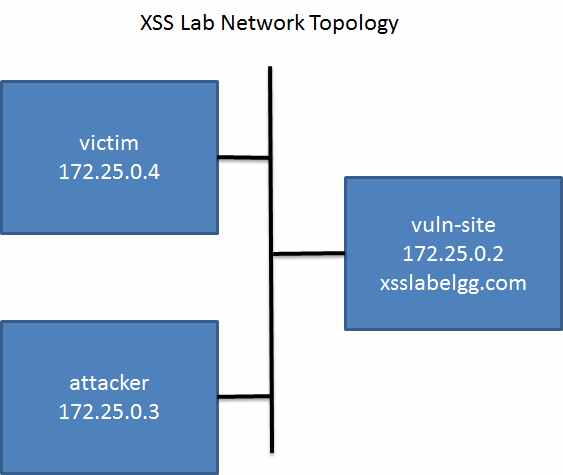
\includegraphics [width=0.8\textwidth,natwidth=621,natheight=403]{xsite.jpg}
\end{center}
\caption{Cross site scripting lab topology}
\label{fig:topology}
\end{figure}


\paragraph{Starting the Apache Server.}
The Apache web server will be running when the lab
commences.  If you need to restart the web server, use
You need to first start the web server using the
the following command:
\begin{verbatim}
   % sudo systemctl restart httpd
\end{verbatim}

\paragraph{The {\tt Elgg} Web Application.}
We use an open-source web application called {\tt Elgg} in this lab.
{\tt Elgg} is a web-based social-networking application. 
It is already set up in on the vuln-server.
We have also created several user accounts on the {\tt Elgg} server and the credentials are given below.


\vspace{0.1in}
\begin{tabular}{|l|l|l|}
\hline
User 	& UserName 	& Password\\
\hline
Admin 	& admin 	& seedelgg \\
Alice 	& alice 	& seedalice \\
Boby 	& boby 		& seedboby \\
Charlie & charlie 	& seedcharlie \\
Samy 	& samy 		& seedsamy \\
\hline
\end{tabular}
\vspace{0.1in}


\paragraph{Configuring DNS.}
We have configured the following \urlorurls needed for this lab: 
